\chapter{Experimental setup}
\label{chap:Experimentalsetup}


\section{Datasets}
\label{sec:datasets}

We use 5 datasets in our experiments, PowerDemand, SMTP, HTTP, SMTP+HTTP and ForestCover, those are widely used streaming datasets in the streaming data mining area \cite{encdecad}\cite{threaded}\cite{tan}. Statistical features are listed in  Table~\ref{tab:dataset}. PowerDemand is a small univariate time series that records the power demand over a period of one year. Weekdays’ demand is higher than weekends’ and daytime is higher than nights, demand of special days (e.g. festivals) are abnormal. We demonstrate a synthetic example with visualization using this dataset while the trends and anomalous states are relative obviously. SMTP, HTTP, SMTP+HTTP are streaming anomaly data extracted from KDD Cup 99 dataset. According to Tan et al. \cite{tan}, HTTP contains sudden surges of anomalies and SMTP does not, but possibly exhibits some distribution changes within the stream. Because of the difficulty to point out where the distribution changes occur in the stream, the HTTP+SMPT dataset is derived by connecting SMTP and HTTP, so that a distribution change is occurred when the communication protocol is switched. The ForestCover dataset is from the UCI repository, which contains 6 kinds of forest cover types. Similar as Dong et al. \cite{threaded}, we defined the smallest class Cottonwood/Willow with 2747 instances as anomaly, and the rest 5 classes as normal class with distribution changes.

\begin{table}[ht] 
\caption{Datasets information} 
\centering      
\begin{tabular}{c c c c}  
\hline\hline        
Dataset & Size & Dimensionality & Anomaly proportion(\textperthousand) \\ [0.5ex] 
\hline 
PowerDemand & 35 040 & 1 &  21.92\\  
SMTP & 96 554 & 41 & 12.25  \\ 
HTTP & 623 091 & 41  & 6.49  \\ 
SMTP+HTTP & 719 645 & 41 & 7.26 \\ 
ForestCover & 581 012 & 32 & 3.53 \\ [1ex]  
\hline    
\end{tabular}
\label{tab:dataset}  
\end{table} 

\section{Data stream configuration}
\label{sec:datastream}

\begin{figure}[h]
\centering
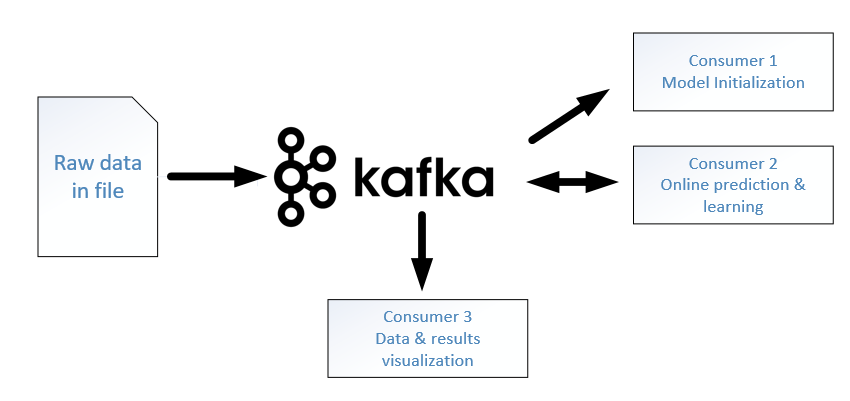
\includegraphics[width=10cm, height=5cm]{kafka}
\caption[Data stream Publisher-Consumer architecture]{Data stream Publisher-Consumer architecture}
\label{fig:kafka}
\end{figure}

\section{Parameter tuning}
\label{sec:parametertuning}

Grid search over: \\
batch size
window length
hidden layer size
epoches


\section{Baseline model}
\label{baseline}
EncdecAD offline










